\documentclass[hyperref={pdfpagelabels=false}, xcolor=dvipsnames]{beamer}
%\usetheme{Copenhagen}
\usepackage{lmodern}
\usepackage{xcolor}
\usepackage{hyperref}

\setbeamercolor{titlelike}{fg=Emerald}
\setbeamercolor{title}{bg=gray!15}
\setbeamercolor{structure}{fg=Emerald}

\title{\textbf{Abschlusspräsentation} \\
        \large PS SWE SS21}
\author{G1T1}

\begin{document}
\maketitle

\begin{frame}
\pagecolor{JungleGreen!10}
\frametitle{Inhalt}
\tableofcontents
\end{frame}

\section{Sequenzdiagramme}
\subsection{Würfelkommunikation}
\begin{frame}
\frametitle{Würfelkommunikation}
\begin{figure}[H]\centering
  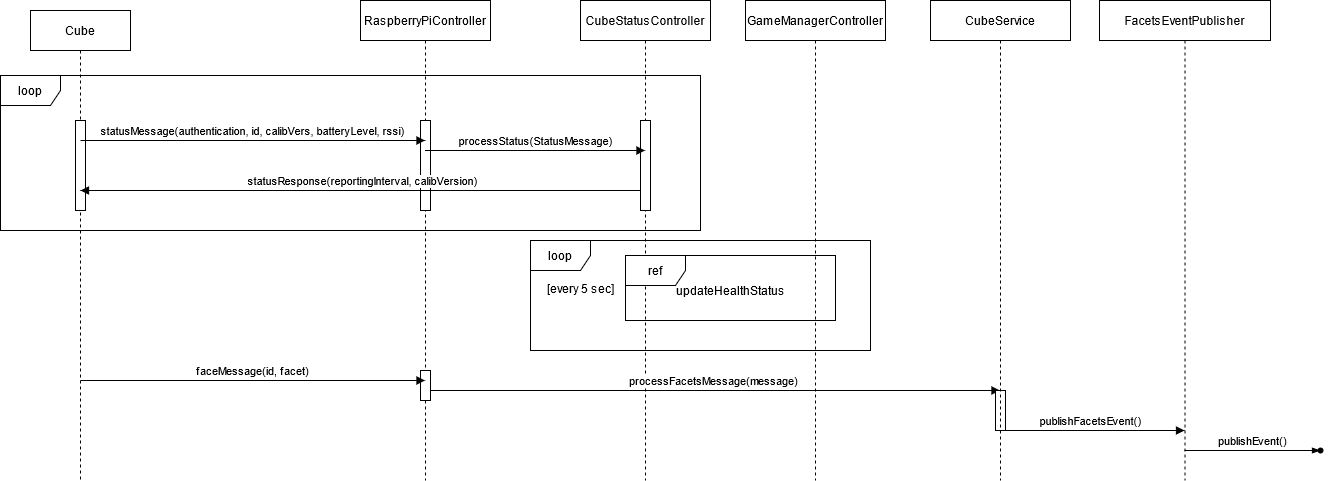
\includegraphics[height=1.5in]{cube0.png}
\end{figure}
\begin{itemize}
  \item \href{file:///C:/Users/cubeCommunication.html}{cubeCommunication.html}
\end{itemize}
\end{frame}

\section{Jacoco-Report}
\begin{frame}
\frametitle{Jacoco-Report}
\begin{figure}[H]\centering
  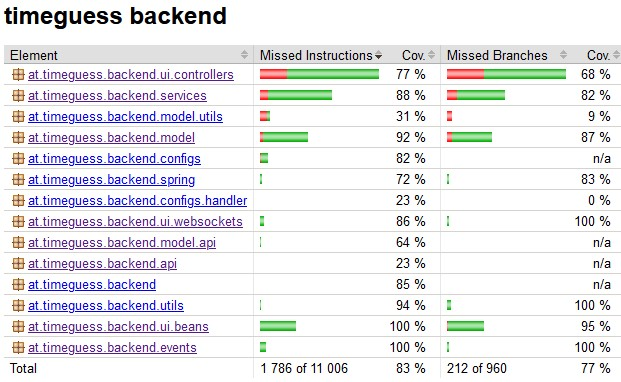
\includegraphics[height=1.9in]{jacoco}
\end{figure}
\begin{itemize}
  \item 757 Testfälle
  \item 83\% Coverage 
\end{itemize}
\end{frame}

\section{Abschlussbericht}
\subsection{Analyse des Projektverlaufs}
\begin{frame}
\frametitle{Analyse des Projektverlaufs / Implementierten Systems}
\begin{itemize}
  \item Projektverlauf erfolgte bis auf kleinere Abweichungen nach den definierten Meilensteinen
  \item Zeitrechnung weicht geringfügig ab: mehr Zeit zum Implentieren wurde benötigt
  \item Initiales Konzept war während der Entwicklung größtenteils stabil: Klassen wurden aber ergänzt
  \item Gesamte geplante Funktionalität konnte umgesetzt werden
  \item Qualitätssicherung durch Tests und gegenseitige Checks der Merge-Requests im GIT 
\end{itemize}
\end{frame}

\subsection{Eingesetzte Werkzeuge}
\begin{frame}
\frametitle{Eingesetzte Werkzeuge}
\begin{itemize}
  \item JSF / Primefaces
  \item GIT
  \item Discord
  \item Docker
  \item Office 365
\end{itemize}
\end{frame}

\section{LIVE-Demo}
\begin{frame}
\frametitle{LIVE-Demo}
\begin{figure}[H]\centering
  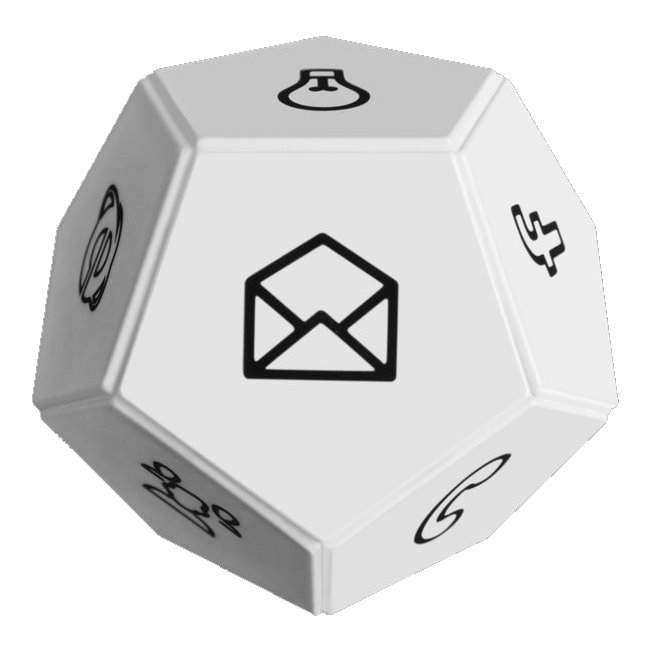
\includegraphics[height=1in]{logo.jpg}
\end{figure}

\begin{itemize}
  \item Host Digital Ocean
  \item \url{http://timeflipgame.online}
\end{itemize}
\end{frame}

\subsection{Ende}
\begin{frame}
\frametitle{Ende}
\centering
\textbf{Danke für die Aufmerksamkeit!}
\end{frame}

\end{document} 